\section{Tolérances aux pannes}

\subsection{Présentation générale}

De manière globale, en plus des différents outils utilisés pour la résilience telle que zookeeper ou haproxy, cette stack dispose d'un serveur globale pour la gestion des pannes. Ce serveur va avoir pour rôle de lancer de manière période des vérifications de status des différents service. Selon les résultats obtenue, le service pourra être redémarré ou même installé sur une nouvelle machine. De plus pour permettre un suivie facile des erreurs de fonctionnement des status, un mail est envoyé dés lors qu'une erreur est détecté. Dans le message du mail est indiqué si l'erreur à put être solutionné de maniére automatique.

\subsection{Infrastructure mise en place}
\ \\
\centerline{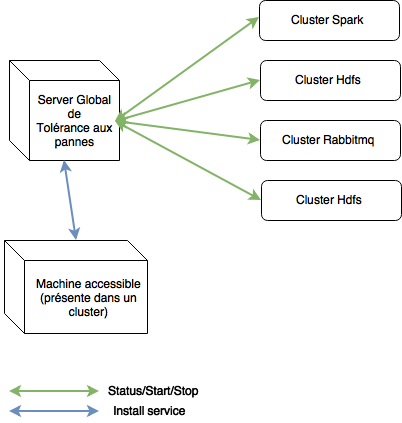
\includegraphics[scale=0.50]{pics/resilience-infra.png}}
\centerline{\caption{Schéma globale de l'infrastructure mise en place pour SPARK}}
\ \\